
%
\documentclass[%
 reprint,
 amsmath,amssymb,
 aps,
]{revtex4-1}

\usepackage{graphicx}% Include figure files
\usepackage{dcolumn}% Align table columns on decimal point
\usepackage{bm}% bold math


\begin{document}



\title{Comparativa Business Intelligence vs Business Analytics}
\author{Richard Cruz Escalante}
\author{Arlyn Cotrado Coaquira}
\author{David Damian Mamani}
\author{Andrés De La Barra Vasquez}
\affiliation{%
 Universidad Privada de Tacna \textbackslash Facultad de Ingenieria \textbackslash Escuela Profesional de Ingenieria de Sistemas
}%

\begin{abstract}
\begin{center}
\textbf{Resumen}
\end{center}

El objetivo de Business Intelligence es permitir que la administración tome decisiones más inteligentes sobre la base del conocimiento extraído de los datos. 
El articulo tambien tiene como objetivo describir los conceptos de business intelligence y business analytics, asi como la comparacion de ellos,  Tambien mencionar las herramientas respectivas.


\begin{center}
\textbf{Abstract}
\end{center}
The objective of Business Intelligence is to allow management to make smarter decisions based on the knowledge extracted from the data.
The article also aims to describe the concepts of business intelligence and business analytics, as well as comparing them, also mention the respective tools.

\end{abstract}



\maketitle

%\tableofcontents

\section {Introducción}


En los últimos años, las organizaciones han recurrido cada vez más a soluciones de software avanzadas para gestionar las cargas de trabajo, mantener la rentabilidad y garantizar la competitividad dentro de sus respectivas industrias. Si bien hay varias opciones disponibles, las herramientas de BI y de BA son posiblemente las soluciones de administración de datos más ampliamente implementadas. \\
Marcar diferencias entre ambos conceptos no es una labor sencilla, porque los dos parten de un mismo principio: el aprovechamiento de la información para tomar mejores decisiones de negocios.

\par El resto de este articulo esta organizado de la siguiente manera. En la Sección 2 se explica el concepto de business intelligence y como se aplica, como tambien sobre business analytics, y la comparación entre business intelligence y analytics. En la Sección 3 se explica el analisis, y finalmente las conclusiones se encuentran en la Sección 4.


%-----------------------------------------------------------------
\section {Marco Teórico}

\subsection{Business Intelligence}

\subsection{Business Analytics}
Hay muchos puntos de vista sobre cómo definir los análisis de negocios, es más que un simple análisis, mientras que las analíticas y las analíticas de negocios a veces se usan indistintamente, tienen focos diferentes. Si bien es esencial, analitycs es solo una parte de la analítica empresarial.
El análisis de negocio(Business Analytics, BA) es el conjunto de métodos y técnicas utilizadas para trabajar como enlace entre los stackeholders, con el fin de comprender la estructura, políticas y operaciones de una organización y recomendar soluciones que permitan a la organización alcanzar sus objetivos (IIBA: International Institute of Business Analysis).\\\\
El análisis de negocios implica la comprensión de cómo funcionan las organizaciones para llevar a cabo sus propósitos, y la definición de las capacidades que una organización requiere para proporcionar productos y servicios a los grupos de interés externos. Incluye la definición de los objetivos de la organización, cómo esos objetivos se conectan a objetivos específicos, que determinan las líneas de acción que una organización tiene que realizar para alcanzar esas metas y objetivos, y definir cómo las distintas unidades de organización y las partes interesadas dentro y fuera de esa organización interactúa.
Aplicaciones del analisis de negocio:
\begin{itemize}
\item Business Intelligence: Conectar a las personas con la información cuándo, dónde y cómo lo necesiten, y colabore para mejorar el rendimiento de negocio.
\item Rendimiento financiero y gestión estratégica: Dirigir la estrategia de gestión hacia los objetivos más rentables mediante información fiable y puntual y la creación de informes transparente y oportuna.
\item Analítica predictiva: Identificar patrones y asociaciones sutiles y desarrollar modelos predictivos para optimizar la toma de decisiones.
\item Gobierno del dato, riesgo y cumplimiento normativo: Obtener un mayor conocimiento en todos los aspectos relacionados con el GRC con una solución integrada cuyos métodos específicos de cumplimiento normativo y de control de riesgos se adaptan a su organización.
\item Aplicaciones analíticas: Proporcionar a los responsables de la línea de negocio el conocimiento accionable con soluciones empaquetadas de análisis y de creación de informes.


	\end{itemize} 

\begin{figure}[htb]
\begin{center}
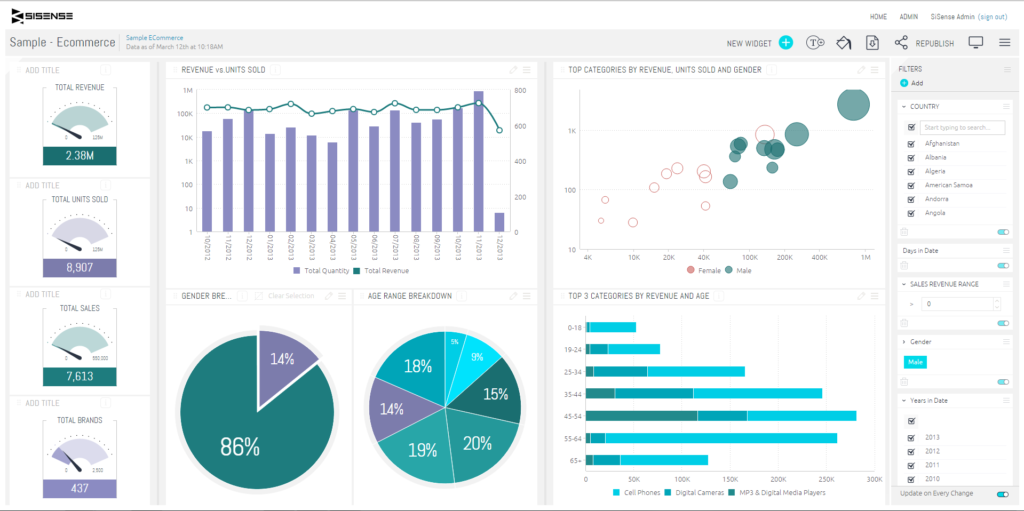
\includegraphics[width=10cm]{./Imagenes/anegocios}
\end{center}
\end{figure}


\subsection{Comparativa}
A continuación, se muestra un cuadro comparativo entre Business Intelligence y Analytics:
\begin{center}
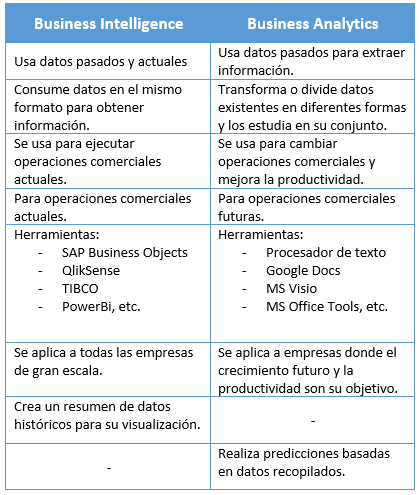
\includegraphics[width=10cm]{./Imagenes/vs1} \cite{hub} \cite{e}
\end{center}

\subsection{Herramientas}
\textbf{Business Intelligence :}
Las herramientas de inteligencia empresarial (BI) son tipos de software de aplicación que recopilan y procesan grandes cantidades de datos no estructurados que proceden de sistemas internos y externos, incluidos libros, publicaciones, documentos, historias clínicas, imágenes, archivos, correo electrónico, vídeos y otros orígenes empresariales. Aunque no son tan flexibles como las herramientas de análisis de negocios, las herramientas de BI ofrecen un modo de acumular datos para encontrar información, principalmente mediante consultas. Estas herramientas también ayudan a preparar los datos para analizarlos con el fin de crear informes, paneles y visualizaciones de datos.\\
\textbf{ Ventajas de las herramientas de Business Intelligence}\\
- La capacidad de analizar de forma combinada información interna y externa procedente de distintas fuentes y sistemas.\\
-Una mayor profundidad de análisis y una capacidad ampliada de reporting.\\
-La posibilidad de remontar ese análisis atrás en el tiempo en base a series históricas.\\
-La capacidad de realizar proyecciones y pronósticos de futuro en base a toda esa información.\\
\begin{itemize}
\item \textbf{IBM Cognos Analytics :}
Es una suite de soluciones de análisis avanzado de información para tomar decisiones: reporting, cuadro de mando, planificación, presupuestación, simulación y análisis cognitivo.
\item \textbf{Microsoft Dynamics :}
Es un sistema de gestión integrada para la empresa, también definido como ERP o Sistema de Planificación de Recursos Empresariales (Enterprise Resource Planning).
\item \textbf{Oracle Business Intelligence :}
Proporciona al usuario un sólido conjunto de informes, consultas ad-hoc, paneles de control y funcionalidad de cuadro de mando. Las soluciones OBIEE son soluciones rentables si la comparamos con una arquitectura orientada a servicios basada en web.
\item \textbf{Style Intelligence:}
Es una plataforma de inteligencia de datos para tableros interactivos, análisis e informes. En su base se encuentra un poderoso motor de mashup de datos que permite una transformación rápida y flexible de datos de fuentes dispares que resuelve los desafíos de administración de datos que otras herramientas de inteligencia empresarial no pueden. Diseñada para una implementación rápida, la aplicación maximiza el autoservicio para una gama de usuarios, desde negocios casuales o navegadores de tipo consumidor hasta usuarios avanzados y científicos de datos.

	\end{itemize} 

\textbf {Business Analytics :}

Las herramientas de análisis de negocios son tipos de software de aplicación que recuperan datos de uno o varios sistemas empresariales y los combinan en un repositorio, como un almacén de datos, para revisarlos y analizarlos. La mayoría de las organizaciones utilizan más de una herramienta de análisis, como hojas de cálculo con funciones estadísticas, paquetes de software estadístico, sofisticadas herramientas de minería de datos y herramientas de modelado predictivo.  Juntas, estas herramientas de análisis de negocios le aportan a la organización una visión completa de la compañía que le permite conocer y comprender el negocio, de modo que pueden tomar mejores decisiones en cuanto a operaciones comerciales, conversiones de clientes, etc.
\\
\textbf{ Ventajas de las herramientas de Business Analytics}\\
- Te permite tener claridad de los atributos positivos internos de la organización y que están bajo control.\\
- Conocer las fortalezas de los recursos con los que cuentas, las ventajas competititvas de tu organización y fuerza de trabajo.\\
- Te ofrece los componentes internos que añaden valor u ofrecen una ventaja competitiva a tu negocio.\\
\textbf{ Desventajas de las herramientas de Business Analytics}\\
- Se basa en los puntos que están bajo el control de la empresa, limitándose sólo al grado de su propia experiencia, que en ocasiones es limitada.\\
- Al centrarse en los aspectos negativos internos, muchas veces no se toma en cuenta cómo repercute en los servicios o productos que proporciona la empresa. Hay que trabajar todo en conjunto.\\

\begin{itemize}

\item \textbf{ Análisis PESTEL: }
Con esta herramienta de análisis estratégico podremos analizar el entorno en el que queremos crear o establecer nuestra empresa, negocio o proyecto. Nos permite identificar posibles cambios de escenario en nuestro sector o en la región para detectar y aprovechar posibles oportunidades de crecimiento.

\includegraphics[width=8cm]{./Imagenes/img1}
\textbf{ Ventajas}\\
. Muestra en un solo informe el entorno de nuestra organización\\
. Descubrimiento de oportunidades y amenazas\\
. Nos ayuda a planificar\\
. Herramienta sencilla de utilizar\\
\textbf{ Desventajas}\\
- Posibilidad de pasar por alto información relevante si no se realiza de manera exhaustiva, hay que dotarlo de un enfoque profundo\\
- Necesidad de actualización periódica, especialmente en sociedades en rápido desarrollo\\
- La información necesaria no siempre es fácil de conseguir (ni barata)\\
- Las estrategias pueden no ser las más convenientes si no se realizan de manera adecuada\\
- Dificultad para establecer modelos sobre lo que va a pasar en el futuro

\item \textbf{ Análisis FODA: }
El análisis FODA es una herramienta de planificación estratégica, diseñada para realizar una análisis interno (Fortalezas y Debilidades) y externo (Oportunidades y Amenazas) en la empresa. Desde este punto de vista la palabra FODA es una sigla creada a partir de cada letra inicial de los términos mencionados anteriormente.
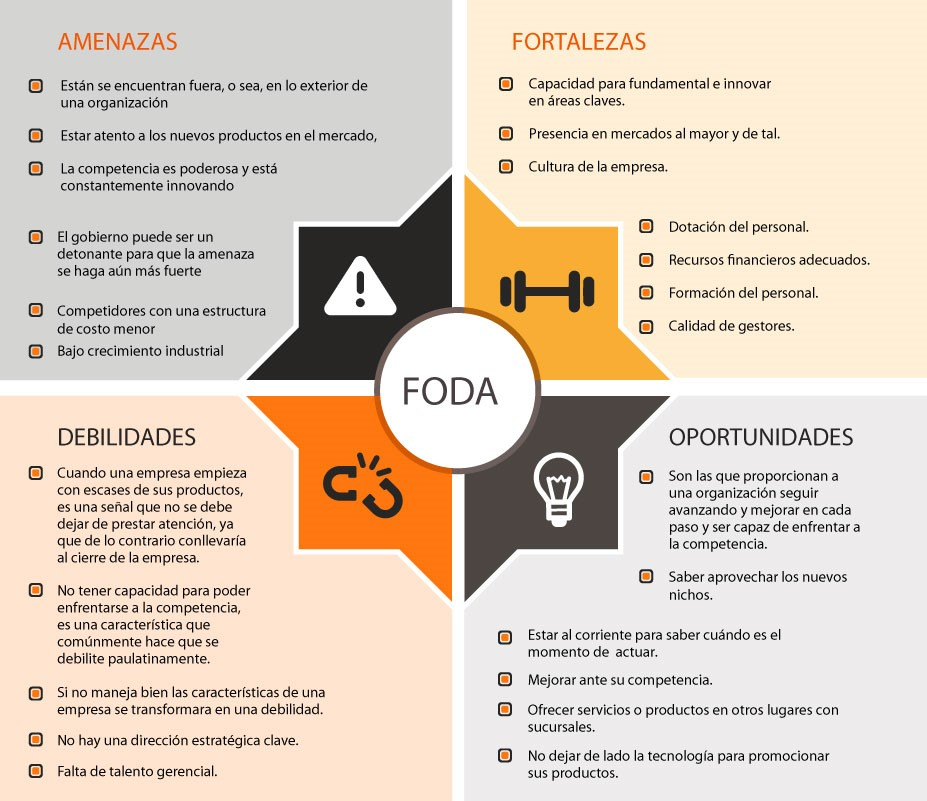
\includegraphics[width=6cm]{./Imagenes/img2}\\
\textbf{ Ventajas}\\
. Muestra en un solo informe el entorno de nuestra organización\\
. Descubrimiento de oportunidades y amenazas\\
. Nos ayuda a planificar\\
. Herramienta sencilla de utilizar\\
\textbf{ Desventajas}\\
. Posibilidad de pasar por alto información relevante si no se realiza de manera exhaustiva, hay que dotarlo de un enfoque profundo\\
. Necesidad de actualización periódica, especialmente en sociedades en rápido desarrollo\\
. La información necesaria no siempre es fácil de conseguir (ni barata)\\
. Las estrategias pueden no ser las más convenientes si no se realizan de manera adecuada\\
. Dificultad para establecer modelos sobre lo que va a pasar en el futuro\\

\item \textbf{ Modelo de las 7 S: }
Las fortaleza de las 7S  es que es una herramienta de diagnostico para entender por qué las organizaciones son ineficaces. Una vez analizados los puntos débiles y realizados cambios, se conduce a un cambio organizacional, implicando al total de la compañía que puede hacer mejorar significativamente su forma de funcionar y sus resultados.
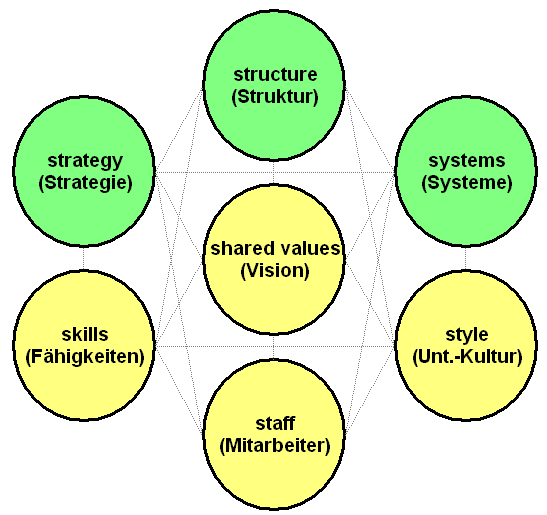
\includegraphics[width=8cm]{./Imagenes/img3}

	\end{itemize} 

%-----------------------------------------------------------------
\section{Análisis}


%-----------------------------------------------------------------
\section{Conclusiones}
\begin{itemize}
\item En forma exclusiva, la inteligencia empresarial y el análisis de negocios forman los componentes esenciales requeridos por una empresa para administrar su información de manera efectiva.
\\
\item 
Las dos terminologías parecen tener similitudes de una manera que hace que los estudiantes deduzcan que están conectados. De hecho, vale la pena reconocer que la analítica es una función de la inteligencia empresarial. La información analizada mediante análisis para predecir el futuro es la misma información obtenida del componente de inteligencia de la empresa. Tanto BI como BA se enfocan en impulsar a la compañía a avanzar enérgicamente
\\
\item En un medio globalizado y audaz como el del mundo empresarial, podemos ver que el entorno en el que la inmensa mayoría de las empresas tiene soportados los procesos de negocio con diferentes sistemas de información y estrategias, los ubica en un mercado tan competitivo como el actual, Hoy se ha convertido en un problema, por lo que la Inteligencia de Negocios se erige como una pieza clave para ser proactivo a la hora de tomar mejores decisiones y de conseguir mejor control de negocio y ventajas que nos diferencien de la competencia.
\\
\item la gran mayoría de empresas no utilizan sistemas de inteligencia empresarial para gestionar sus negocios. Sin embargo, entienden el concpeto y saben que son herramientas muy enriquecedoras para la gestión actual.
\end{itemize} 



% Bibliografia.
%-----------------------------------------------------------------

\bibliographystyle{plain}
\bibliography{Bibliografia}

\end{document}

